\newtcolorbox{taxobox}[1][]{
  enhanced,
  colback=sntPurple!5,
  colbacktitle=sntPurple,
  coltitle=white,
  sharp corners,
  frame hidden,
  boxrule=0pt,
  fontupper=\small,
  fonttitle=\centering\bfseries\scshape,
  after title app=\strut,
  height=3.5cm,
  title=#1
}

\subsection[\eiffel Assessment \& \texttt{eiffel}]{\texorpdfstring{\eiffel Assessing the Impact of Label-Flipping Attacks}{Assessing the Impact of Label-Flipping Attacks}}



\begin{frame}{The Problem of Poisoning Attacks}
  \stepcounter{beamerpauses}
  \begin{columns}
    \column{.5\textwidth}
    \begin{block}{Definition}
      Manipulation of the training data or model updates cause unwanted behaviors in the aggregated model.
    \end{block}

    \column{.5\textwidth}
    \onslide<1->{
      \begin{figure}
        \centering
        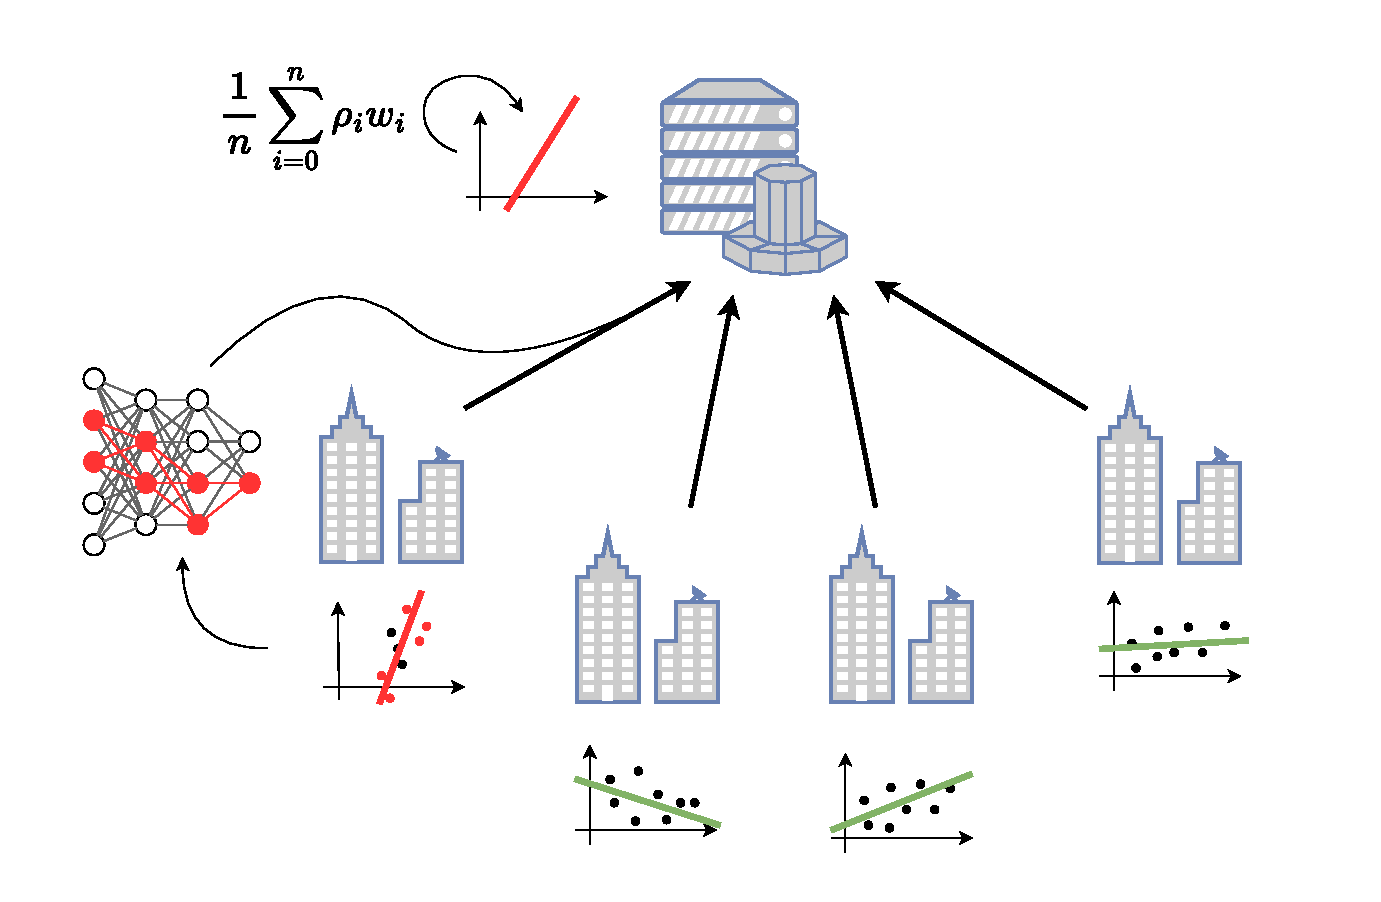
\includegraphics[width=\textwidth,trim={0 1cm 0 1cm},clip]{figures/thesis/assessment/poisoning/6.pdf}
        \caption{Poisoning attacks on FL.}
    \end{figure}}
  \end{columns}

  \alt<2->{\footcite*{lavaur_cose_2025}}{\blankfootnote{\newline}}
\end{frame}













